\documentclass[conference]{IEEEtran}
\IEEEoverridecommandlockouts

\usepackage[british]{babel}
\usepackage[noadjust]{cite}
\usepackage{graphicx}
\usepackage[hyphens]{url}
\usepackage{paralist}
\usepackage{booktabs}
\usepackage[pdftex,colorlinks=true]{hyperref}

% reduce indent on all paralist environments
%\setdefaultleftmargin{0.5cm}{}{}{}{}{}

\begin{document}

% paper title
\title{Engagement and Interactions of Language Communities on Twitter}


% author names and affiliations
% use a multiple column layout for up to three different
% affiliations
\author{\IEEEauthorblockN{Nabeel Albishry}
\IEEEauthorblockA{Department of Computer Science\\
University of Bristol\\
Bristol, UK\\
Email: n.albishry@bristol.ac.uk}
\and
\IEEEauthorblockN{Theo Tryfonas}
\IEEEauthorblockA{Department of Civil Engineering\\
University of Bristol\\
Bristol, UK\\
Email: theo.tryfonas@bristol.ac.uk}
\and
\IEEEauthorblockN{Tom Crick}
\IEEEauthorblockA{Department of Computing\\
Cardiff Metropolitan University\\
Cardiff, UK\\
Email: tcrick@cardiffmet.ac.uk}}

% conference papers do not typically use \thanks and this command
% is locked out in conference mode. If really needed, such as for
% the acknowledgment of grants, issue a \IEEEoverridecommandlockouts
% after \documentclass

% use for special paper notices
%\IEEEspecialpapernotice{(Invited Paper)}

% make the title area
\maketitle


\begin{abstract}
In this paper we present our analysis of online conversations that
took place on the social networking site Twitter during the Baltimore
riots in April 2015. It aims to evaluate the extent to which different
language communities engage and interact and thereby utilising
language information from user profiles and statuses to identify and
categorise communities, the pattern of their interactions, and to
construct their network graphs. The results show that the nature of
the event is reflected on the engagement degree and wider interaction
of communities.  This analysis of language communities may also help
in deciding which group of users to engage with, and hence increase
the chance of influential action when participating on Twitter
conversations.
\end{abstract}

% For peer review papers, you can put extra information on the cover
% page as needed:
% \ifCLASSOPTIONpeerreview
% \begin{center} \bfseries Keywords \end{center}
% \fi
%
% For peerreview papers, this IEEEtran command inserts a page break and
% creates the second title. It will be ignored for other modes.
%\IEEEpeerreviewmaketitle

% tweak these at the end
\begin{IEEEkeywords}
Language communities, community interactions, networks, social networking, Twitter.
\end{IEEEkeywords}


\section{Introduction}\label{intro}

Online social networks (OSNs) have been utilised as means to express
opinions, spread information about events, or even stimulate and
propagate calls to action. Social networks such as Twitter played an
important role during what was then known as the ``Arab Spring'',
which has been extensively examined in the social network analysis
domain~\cite{lotan-et-al:2011,howard-et-al:2011,comunello+anzera:2012,wolfsfeld-et-al:2013}. Furthermore,
there are various projects that used Twitter corpora and related
datasets to make predictions about elections~\cite{
tumasjan-et-al:2010}, stock markets~\cite{zhang-et-al:2011}, and
crimes and
policing~\cite{gerber:2014,oatley+crick_fosintsi2014,oatley+crick:2015}.

In the social network analysis (SNA) domain, centrality measures
provide the ability to assess network graphs that are constructed from
collected data (for example, tweets). Selection of these centrality
measures is dependent on the goal of the analysis; for example, the
degree of node helps to identify nodes with high number of connections
within the network. In a representation of a real world network, this
metric may help to identify highly connected persons, such as
political leaders, sports stars or celebrities, who are potential``
information
spreaders''~\cite{cha-et-al:2012,borge-holthoefer-et-al:2012,zhang-et-al:2016}. Centrality
measures such as degrees, betweenness, clustering coefficient,
modularity and cliques have been used in many projects to measure
influence or detect the emergence of new
communities~\cite{willis-et-al:2015,oatley+crick:2015}.

Clustering users in communities has been an important analytic factor
in social networking analysis. Numerous papers have focused on
clustering users based on their locations. However, for sake of
anonymity, many users tend not to disclose information about their
identity, such as locations~\cite{kang-et-al:2013}. It has also been
reported in the literature that geotagged tweets are generally low in
number~\cite{morstatter-et-al:2013}[10][11].

% should this be in the Introduction?
Furthermore, we took the step to verify this claim in our datasets
too. In the best cases, the ratio of geotagged tweets did not exceed
2\%. In the case of the {\texttt{\#BaltimoreRiots}} dataset, only ~1\%
of collected statuses were associated with places. Moreover, out of
this geotagged subset, only 4\% were associated with the city where
the event took place, i.e. Baltimore.

It is important to highlight how geotagging works in Twitter. The
`place' entity included in a Twitter status does not necessarily
indicate precisely where the actual posting was made, as stated in the
Twitter documentation:

\begin{quotation}
``{\emph{Tweets associated with places are not necessarily issued from that
location but could also potentially be about that location.}}'' [12]
\end{quotation}

An alternative location-based option to consider is based on profile
location, but it still does not serve the need for location clustering
for a multitude of reasons. Firstly, we found that less than 45\% of
users have set their profile location, which is in line with other
studies [13]. Secondly, although Twitter suggests certain presets for
setting profile location, users are given the option to enter any text
they wish; this results in a considerable amount of noise.

The techniques we present in this paper are based on language settings
in users' profiles and those for statuses\footnote{The term `status'
is a generic term used to refer to any Twitter post (tweet, retweet,
reply, or quote).}. The remainder of this paper is organised as
follows: Section II introduces the context of the real world situation
and the development of events in alignment with activity on
Twitter. Then in Section III we present the techniques we used and
their results and discussion. Finally, Section IV concludes with
highlights on the potential application of our approach.


\section{Context and Events Timeline}\label{context}

Following the peaceful funeral of Freddie Gray that took place on the
morning of Monday 27 April 2015 in Baltimore, Maryland, USA, a protest
hit the city. According to the timeline published on the CNN website
``{\emph{The city exploded on Monday after the funeral of Freddie
Gray, a 25-year-old black man who mysteriously died on April 19, a
week after Baltimore Police arrested him.}}'' [15]. The nature of the
Baltimore riots is a good representation of a planned event in which a
sudden escalation of violence hits a geographical area. The event
manifested itself on Twitter as {\texttt{\#BaltimoreRiots}}, and
resulted in more than 1,250,000 status updates.

Figure~\ref{fig:overallactivity} and Figure~\ref{fig:mainevents}
present how the event manifested itself on Twitter once a ``purge'' was
scheduled. We can see that what was happening on the ground was
quickly reflected on the activity in Twitter, as
Figure~\ref{fig:mainevents} indicates. More detailed analysis reveals
that within one hour the topic started to go ``viral''; more
precisely, at approximately 15:00 at which the ``purge'' was
scheduled. The topic jumped from roughly 1,200 to 8,000 tweets per
hour. Then, it peaked with 98,000 between 22:00 and 23:00.

\begin{figure}[!htb]
\centering
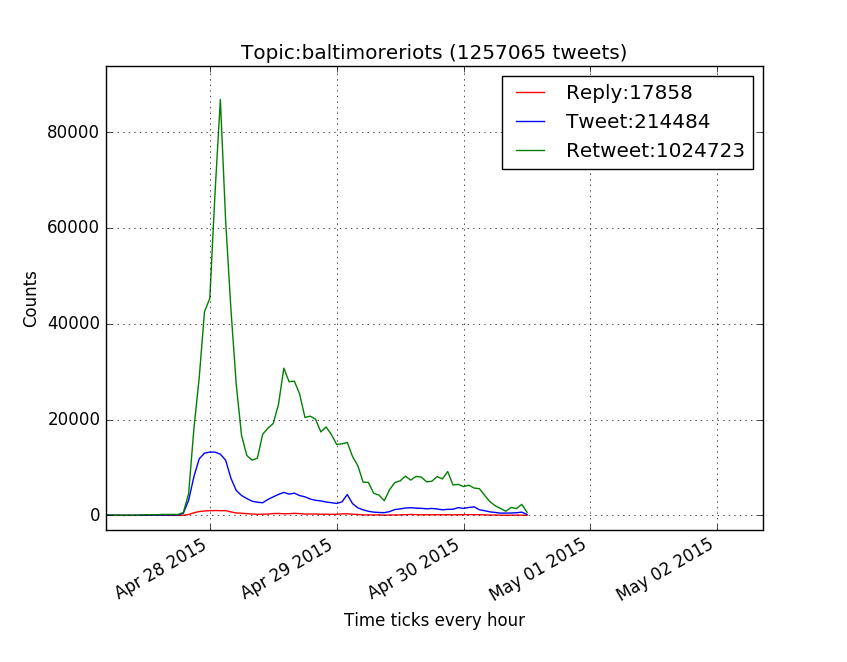
\includegraphics[width=\columnwidth]{images/overallactivity.png}
\caption{Overall activity for {\texttt{\#BaltimoreRiots}}.}
\label{fig:overallactivity}
\end{figure}

\begin{figure}[!htb]
\centering
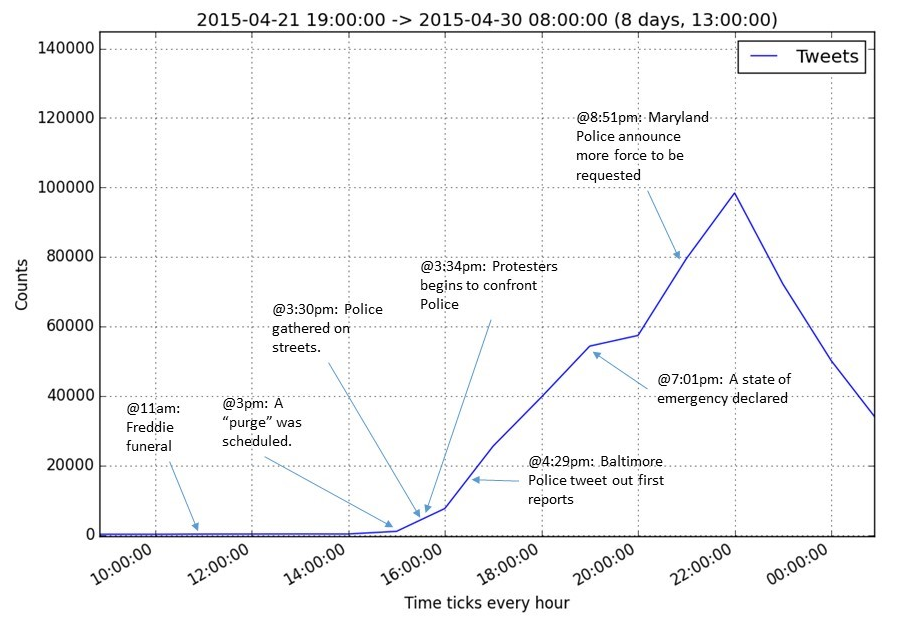
\includegraphics[width=\columnwidth]{images/mainevents.png}
\caption{Main events during the lifetime of {\texttt{\#BaltimoreRiots}}.}
\label{fig:mainevents}
\end{figure}


\section{Language Communities}\label{langcomm}

Analysis of language communities begins with two basic techniques. The
first is to classify statuses based on their languages. The status
language is extracted from the `lang' entity inside status
objects. Language used in posting defines which community the status
was meant for; a tweet written in Turkish, for example, is meant for
the Turkish-speaking community. Output from this will be referred to
as `posting communities'. The second analysis is to classify users
into different communities based on their profile languages,
regardless of the posting language they used. Output from this
technique will be referred to as `profile communities'. As we will see
in the following sections, a posting community does not necessarily
indicate the profile community for a user. Therefore, the second step
is to examine the relationship between profile and posting
communities. We will also explore relationships amongst profile
communities, in term of action-reaction. We will investigate the
intra- and inter-profile communities interactions by constructing
network graphs and generate a visual representation.

\subsection{Posting Communities}

In the {\texttt{\#BaltimoreRiots}} case, there were 38 posting
languages. As we can see in Figure~\ref{fig:langfreq}, English was the
dominating language by far. Interestingly, results also show that
language of more than 41,000 (~3\%) statuses could not be
identified. When investigated, those statuses mostly do not contain
text other than hashtags, pictures or URLs. Although, this is not a
big portion, it came second after English. Although this category
shows an interesting case in which qualitative content analysis would
be involved, it is beyond this study and will not be covered here.

\begin{figure}[!htb]
\centering
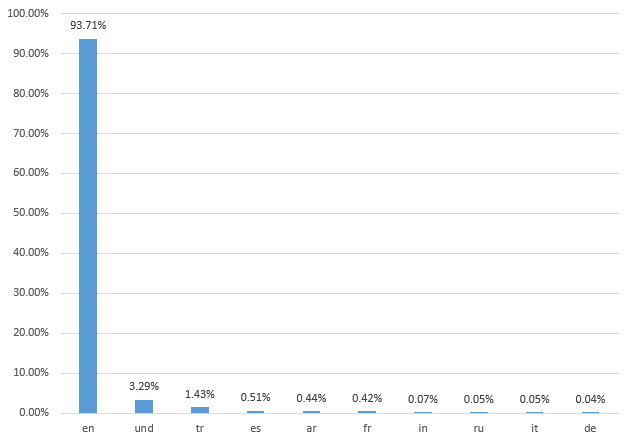
\includegraphics[width=\columnwidth]{images/langfreq.png}
\caption{Most frequently used languages in {\texttt{\#BaltimoreRiots}}
  (en: English, es: Spanish, tr: Turkish, fr: French, en-gb: English
  United Kingdom, ar: Arabic, de: German, ru: Russian, it: Italian,
  pt: Portuguese)}
\label{fig:langfreq}
\end{figure}


\subsection{Users' Language Communities}

In the majority of cases, users choose to pick a language for their
Twitter profile settings. In our dataset we found that out of 716,494
users, only 45 had not chosen any language. However, the language
entity returned by the API for those cases is the initial placeholder
text ``Select Language...'' or a translated version that might provide
hints regarding the user language
community. Figure~\ref{fig:activecomm} shows that about 94\% of the
users came from `en' profile community.

\begin{figure}[!htb]
\centering
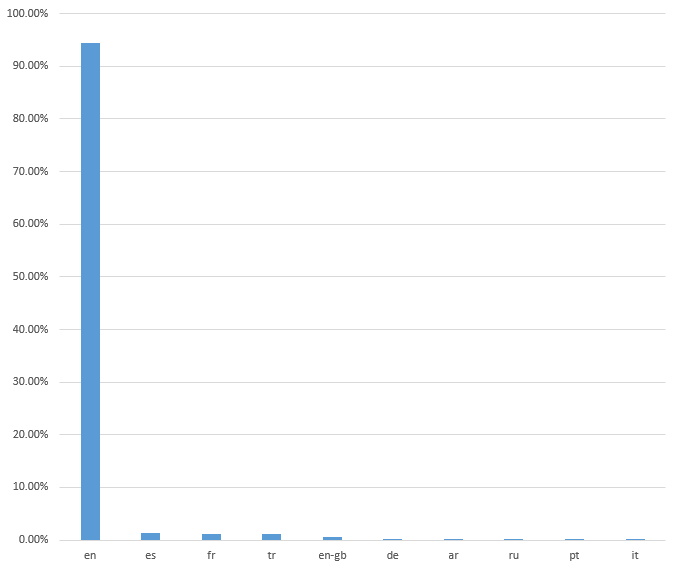
\includegraphics[width=\columnwidth]{images/activecomm.png}
\caption{Top 10 most active communities in {\texttt{\#BaltimoreRiots}}}
\label{fig:activecomm}
\end{figure}

From these two outputs, we can see that nearly all of the topic
activity came from one particular community using one particular
language. This extreme pattern may accompany extreme and
geographically constrained real world events such as riots and terror
attacks.


\subsection{Profile-Posting Graph}

To investigate whether the `en' posting community is linked to
particular profile communities, we constructed a bipartite graph as
presented in Figure~\ref{fig:profilepostinggraph}, representing the
profile-posting language network. In this graph, nodes that are
prefixed by ``{\emph{p\_}}'' represent profile language community, and
nodes that are prefixed by ``{\emph{s\_}}'' represent status language
community. Size of node represents the weighted degree, whereas colour
represents the outdegree; the darker the colour, the higher
outdegree. The graph confirms the domination pattern we highlighted
earlier; furthermore, it shows the relationships between the profile and
posting communities. 

\begin{figure*}[!htb]
\centering
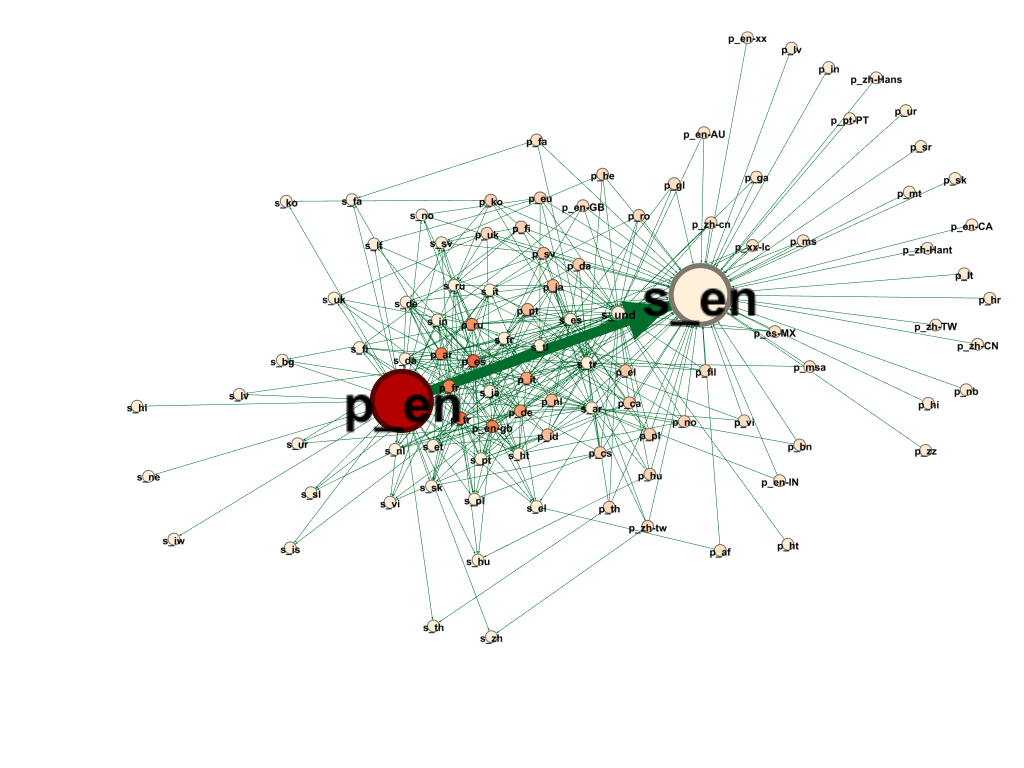
\includegraphics[width=\textwidth]{images/profilepostinggraph.png}
\caption{Profile-posting network graph}
\label{fig:profilepostinggraph}
\end{figure*}

For an extreme case of one dominating posting language, we wanted to
investigate participation of different communities. We thus filtered
out all non-`en' statuses, and then identified different profile
communities with the resultant set. For each community, we classified
statuses into two sets: {\emph{actions}} and {\emph{reactions}}; this
result is shown in Table~\ref{tbl:mostactive}. This shows the highest
scoring communities, where the first column represents the category of
status (action or reaction), community column represents profile
language community, and last one shows percentage of `en’ posts by
that community.

\begin{table}[!htb]
\centering
\begin{tabular}{@{}lcr@{}}
\toprule
\textbf{Category} & \textbf{Community} & \textbf{\%} \\ \midrule
Reaction & en & 81.08 \\
Action & en & 15.43 \\
Reaction & es & 0.68 \\
Reaction & fr & 0.59 \\
Reaction & en-gb & 0.47 \\
Reaction & tr & 0.19 \\
Reaction & de & 0.18 \\
Reaction & pt & 0.13 \\ \bottomrule
\end{tabular}
\caption{Activity and categories of most active profile language
  communities}
\label{tbl:mostactive}
\end{table}

From the results above we can infer that there is a dominating player
in both domains: posting languages and profile communities. Therefore,
for the case of {\texttt{\#BaltimoreRiots}}, we can conclude that the case was
substantially localised.


\subsection{Temporal Communities Activity}

We wished to explore communities' activity over time, apart from the
overall activity. Figure~\ref{fig:heatmap} represents a heat map for
posts per hour for each profile community over the lifetime of
{\texttt{\#BaltimoreRiots}}. This sort of mapping would help in
identifying times at which communities are active.

When refined with posting language, this technique would be useful in
identifying when to engage into conversations, which language
community to target, and by which language. For example, presuming
that we want to participate in a trending topic hashtag that we are
interested in; this analysis technique could help us make our post
more direct and focused. By finding which language is mostly used in
posting, we will be able to know in which language the tweet would be
more effective. Also, we might want to direct the message to certain
language community, be that to influence a very active or re-activate
a quiet one.

\begin{figure*}[!htb]
\centering
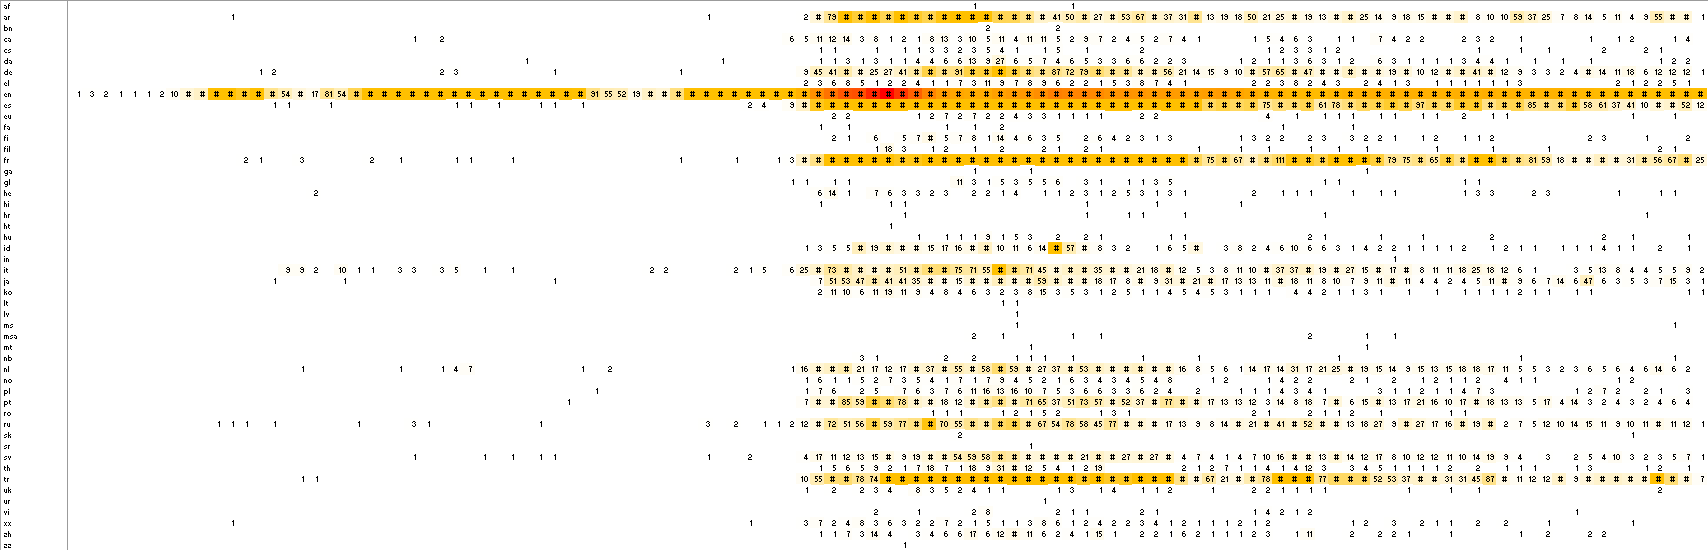
\includegraphics[width=\textwidth]{images/heatmap.png}
\caption{Temporal activity of profile communities}
\label{fig:heatmap}
\end{figure*}


\subsection{Reaction Networks}

Another important perspective to identify and capture is how different
profile communities relate to each other in terms of
reactions. Therefore, we constructed the graph in
Figure~\ref{fig:profileprofilegraph} to show interactions amongst
language communities. Edges are directed and are drawn from reacting
nodes (retweeter, or replier) to the original acting node
(tweeter). As we are not interested in reactions from community to
itself, we eliminated self-loop edges from the graph. Node size
represents weighted indegree.

\begin{figure*}[!htb]
\centering
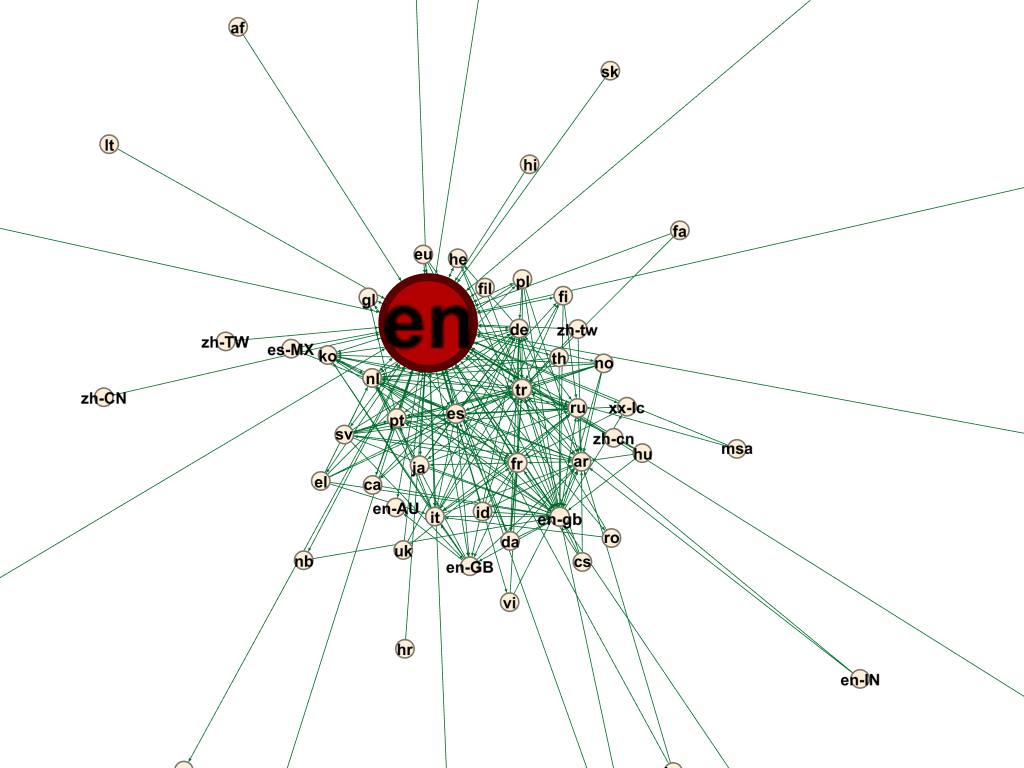
\includegraphics[width=\textwidth]{images/profileprofilegraph.png}
\caption{Profile-profile network graph}
\label{fig:profileprofilegraph}
\end{figure*}


\section{Conclusions}\label{conclusions}

This paper presented a study in identifying languages used, language
communities and their engagement and interactions on the Twitter
platform with respect to real world events. As we discussed in
Section~\ref{langcomm}, the nature of the event (e.g. being a local or
global) may be reflected on community conversations on Twitter. We
found that most of posting activity comes from the main community (the
language community in which the incident has happened or tightly
related to). This is especially the case when the online conversations
are triggered by a real world incident. The same for posting
languages, users mostly to use the language of the main
community. Although most of topic activity comes from that main
community, we noticed that, with local events, other communities work,
mostly, as information spreaders.

We also presented a network graph showing how language communities
relate to each other in the form of action-reaction (action: tweet,
reaction: retweet, reply, quote). Another interesting graph that we
produced to show relations between profile and posting communities. We
find that this graph is important to facilitate comparing users
defined profile language with their posting language. Some event might
be termed as `partially scheduled' as their end was different to how
they were planned in the first place. In such tense situation, we
noticed that diversity of languages and communities are very low, and
there always be a dominating community and language. 

The method we presented here can be used in identifying how
communities interact with one another, which ones are most active,
which languages are mostly used, and at what time. Applying these
techniques on data pouring from the Twitter Stream
API\footnote{\url{https://dev.twitter.com/streaming/overview}} would
be applicable to a wide number of domains. For example, these methods
can be used in social network marketing and publicity to increase the
probability of influential posts. In practice, for a given
{\texttt{\#<Brand>}}, by monitoring the activity of different
language community, one can decide the time to post well-tailored
tweets targeting certain communities. This can be fine-tuned further
by mentioning key players in that community, e.g. users with high
closeness scores.






%\newpage

% trigger a \newpage just before the given reference
% number - used to balance the columns on the last page
% adjust value as needed - may need to be readjusted if
% the document is modified later
%\IEEEtriggeratref{28}
% The "triggered" command can be changed if desired:
%\IEEEtriggercmd{\enlargethispage{-5in}}

% references section
\bibliographystyle{IEEEtran}
\bibliography{ssci2016}

% that's all folks
\end{document}


